\sloppy
\documentclass[14pt,a4paper,oneside]{extarticle}	% Размер основного шрифта и формата листа
\usepackage{xltxtra}						% Используется для вывода логотипа XeLaTeX
\usepackage{xunicode}						% Кодировка документа
\usepackage{polyglossia}					% Загружает пакет многоязыковой верстки
\newfontfamily\russianfont{Book Antiqua}
%\setmainfont{Liberation Serif}						% Основной шрифт текста
\setmainfont{Book Antiqua}
\setdefaultlanguage{russian}				% Основной язык текста
\setotherlanguage{english}					% Дополнительный язык текста
\linespread{1}							% Межстрочный интервал выбран полуторным
\usepackage[left=2.5cm,
right=1.5cm,vmargin=2.5cm]{geometry} % Отступы по краям листа
\bibliographystyle{ugost2008}

\usepackage{xcolor}
\usepackage{hyperref}
% Цвета для гиперссылок
\definecolor{linkcolor}{HTML}{359B08} % цвет ссылок
\definecolor{urlcolor}{HTML}{799B03} % цвет гиперссылок
\hypersetup{pdfstartview=FitH,  linkcolor=linkcolor,urlcolor=urlcolor, colorlinks=true}

%---------------------------%
%---- Пакеты расширений ----%
%---------------------------%
\usepackage{xcolor}
\usepackage{hyperref}
% Цвета для гиперссылок
\definecolor{linkcolor}{HTML}{359B08} % цвет ссылок
\definecolor{urlcolor}{HTML}{799B03} % цвет гиперссылок
\hypersetup{pdfstartview=FitH,  linkcolor=linkcolor,urlcolor=urlcolor, colorlinks=true}


\usepackage{verbatim,indentfirst}
\usepackage{cite,enumerate,float}
\usepackage{amsmath,amssymb,amsthm,amsfonts}

%---------------------------%
%--- Вставка иллюстраций ---%
%---------------------------%
\usepackage{graphicx}
\usepackage{subfigure}
%\graphicspath{{Images/}}
\usepackage{fontspec}

\begin{document}
%	\pagestyle{empty} %  выключаенм нумерацию
%\setcounter{page}{3}% Нумерация начинается с третьей страницы
%\renewcommand{\contentsname}{\center{Содержание}}
%\tableofcontents

\begin{center}
	%\addcontentsline{toc}{section}{Опыт 12. Параболическая поверхность вращающейся жидкости}
	\subsection*{Параболическая поверхность вращающейся жидкости}
\end{center}

\begin{figure}[H]
	\centering 	
	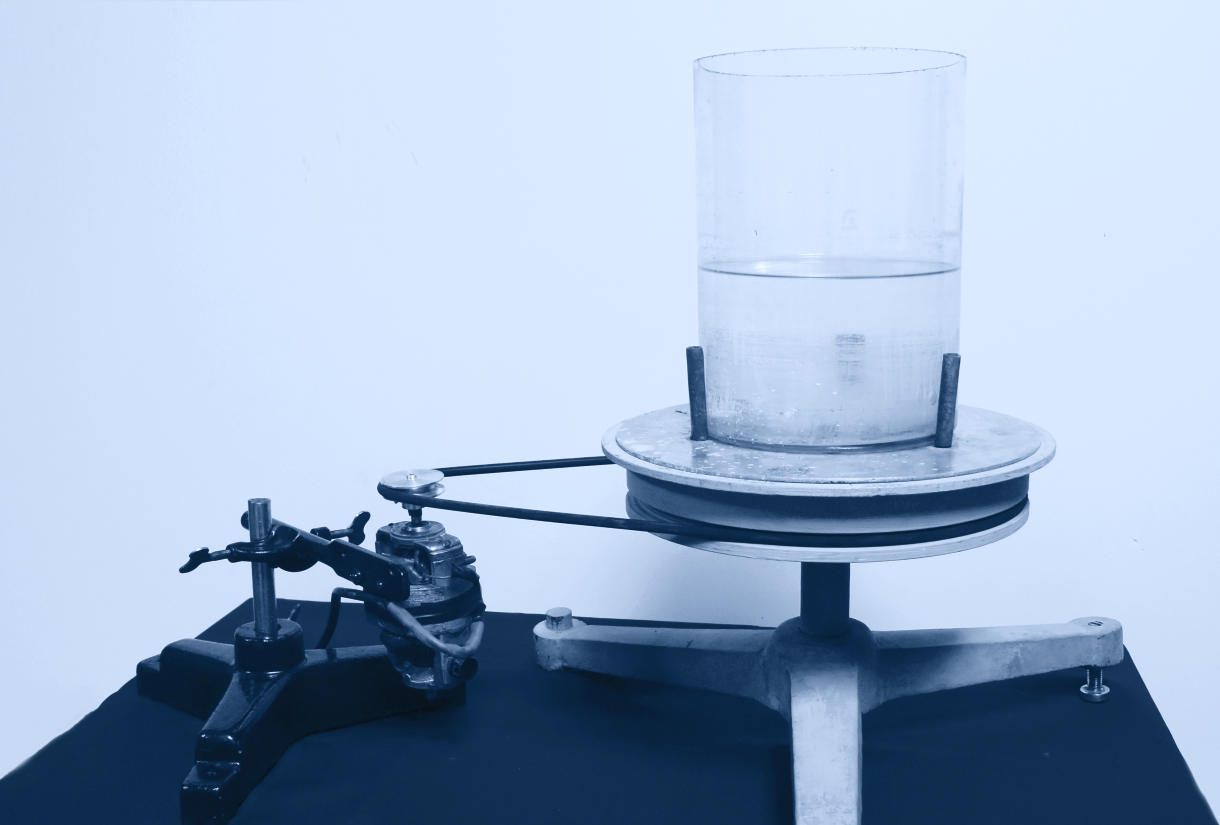
\includegraphics[width=0.9\linewidth]{paraboloid-1.png}
	\caption{Демонстрация параболического профиля при вращении жидкости}
	\label{paraboloid-1}
\end{figure}

\subsection*{\underline{Оборудование:}}

\begin{enumerate}
	\item Стеклянный цилиндрический сосуд диаметром 15 и высотой 30 см.
	\item Жидкость, подкрашенная флуоресцеином.
	\item Вращающаяся платформа.
	\item Электродвигатель с ременной передачей.
	\item Лампа накаливания.
\end{enumerate}

\subsection*{\underline{Основные определения:}}

Поверхностями равного давления называются поверхности с одинаковыми во всех точках давлениями.
Любая горизонтальная плоскость, проведенная в покоящейся жидкости, находящейся под действием силы тяжести, является поверхностью равного давления.

Свободной поверхностью называют плоскость раздела между жидкостью и газообразной средой.
Равнодействующая всех сил, приложенных к каждой частице, лежащей на свободной поверхности покоящейся жидкости, нормальна к этой поверхности.

Относительным равновесием жидкости называется такое состояние, при котором отдельные ее частицы не смещаются одна относительно другой, 
а также стенок сосуда — и вся масса жидкости движется как твердое тело.

В абсолютно покоящейся жидкости (сосуд неподвижен) действующей массовой силой (в поле сил тяжести) является только сила тяжести.
При относительном покое к ней добавляется еще одна массовая сила — сила инерции.

Законы относительного равновесия жидкости находят широкое применение в промышленности, а именно, в измерительной технике (жидкостные тахометры), в металлургии (центробежное литье) и других областях техники.
При изучении относительного равновесия необходимо заниматься, во-первых, установлением закона распределения давления внутри жидкости, 
а, во-вторых, определением формы поверхности равного давления, т.е. такой поверхности, все точки которой испытывают одинаковое давление.

\subsection*{\underline{Краткое описание:}}

На шкив центробежной машины устанавливается подставка с большим цилиндрическим стеклянным стаканом, 
в который примерно до 1/3 его высоты налита слегка подкрашенная вода.
Стакан вращают вначале медленно, а затем, по мере того как вода приходит во вращение, скорость постепенно увеличивают. 
Через некоторое время поверхность воды принимает форму параболоида, что достаточно хорошо видно аудитории, если за стаканом поместить лист белого картона и освещать стакан сверху лампой. 
Для большей наглядности опыта рекомендуется пользоваться чистой водой, 
осветив вращающийся стакан сверху лампой с абажуром. 
Когда поверхность воды примет форму параболоида, следует налить на нее сверху немного раствора флюоресцеина. 
В этом случае параболоид ясно виден вследствие яркого свечения (рис.\ref{paraboloid-2}).

При постепенном повышении скорости центробежная сила инерции, действующая на элементы жидкости, заставляет жидкость прижиматься к стенкам сосуда и свободная поверхность принимает вид параболоида. 

\begin{figure}[H] 	
	\centering 	
	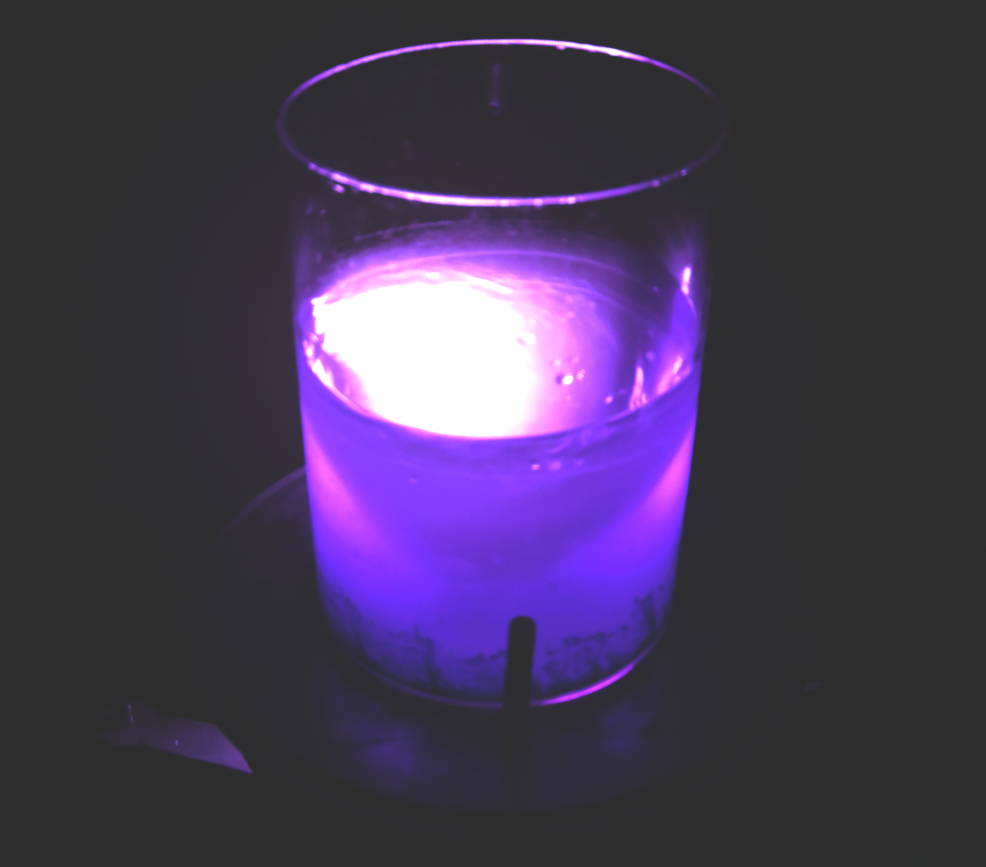
\includegraphics[width=0.6\linewidth]{paraboloid-2.png}
	\caption{Демонстрация поведения жидкости при вращении. Под действием сил инерции свободная поверхность жидкости при ее вращении принимает вид параболоида. Благодаря вязкости и эффекту прилипания к стенкам сосуда жидкость движется как твердое тело и профиль свободной поверхности при равномерном вращении платформы со временем сохраняется}
	\label{paraboloid-2}
\end{figure}


\subsection*{\underline{Теория:}}

Можно установить связь между высотой столба жидкости $ h_{0} $ в сосуде при отсутствии вращения и величинами $ h_{min} $ и $ h_{max} $ при вращении с угловой скоростью $ \omega $ (рис.\ref{paraboloid-3})
\begin{align}\label{1}
h_{max} = h_{0} + \frac{\omega^{2} r^{2}}{4g}, \\
h_{min} = h_{0} - \frac{\omega^{2} r^{2}}{4g},
\end{align}
где \textit{r} — радиус цилиндрического сосуда.

\begin{figure}[H] 
	\centering 	
	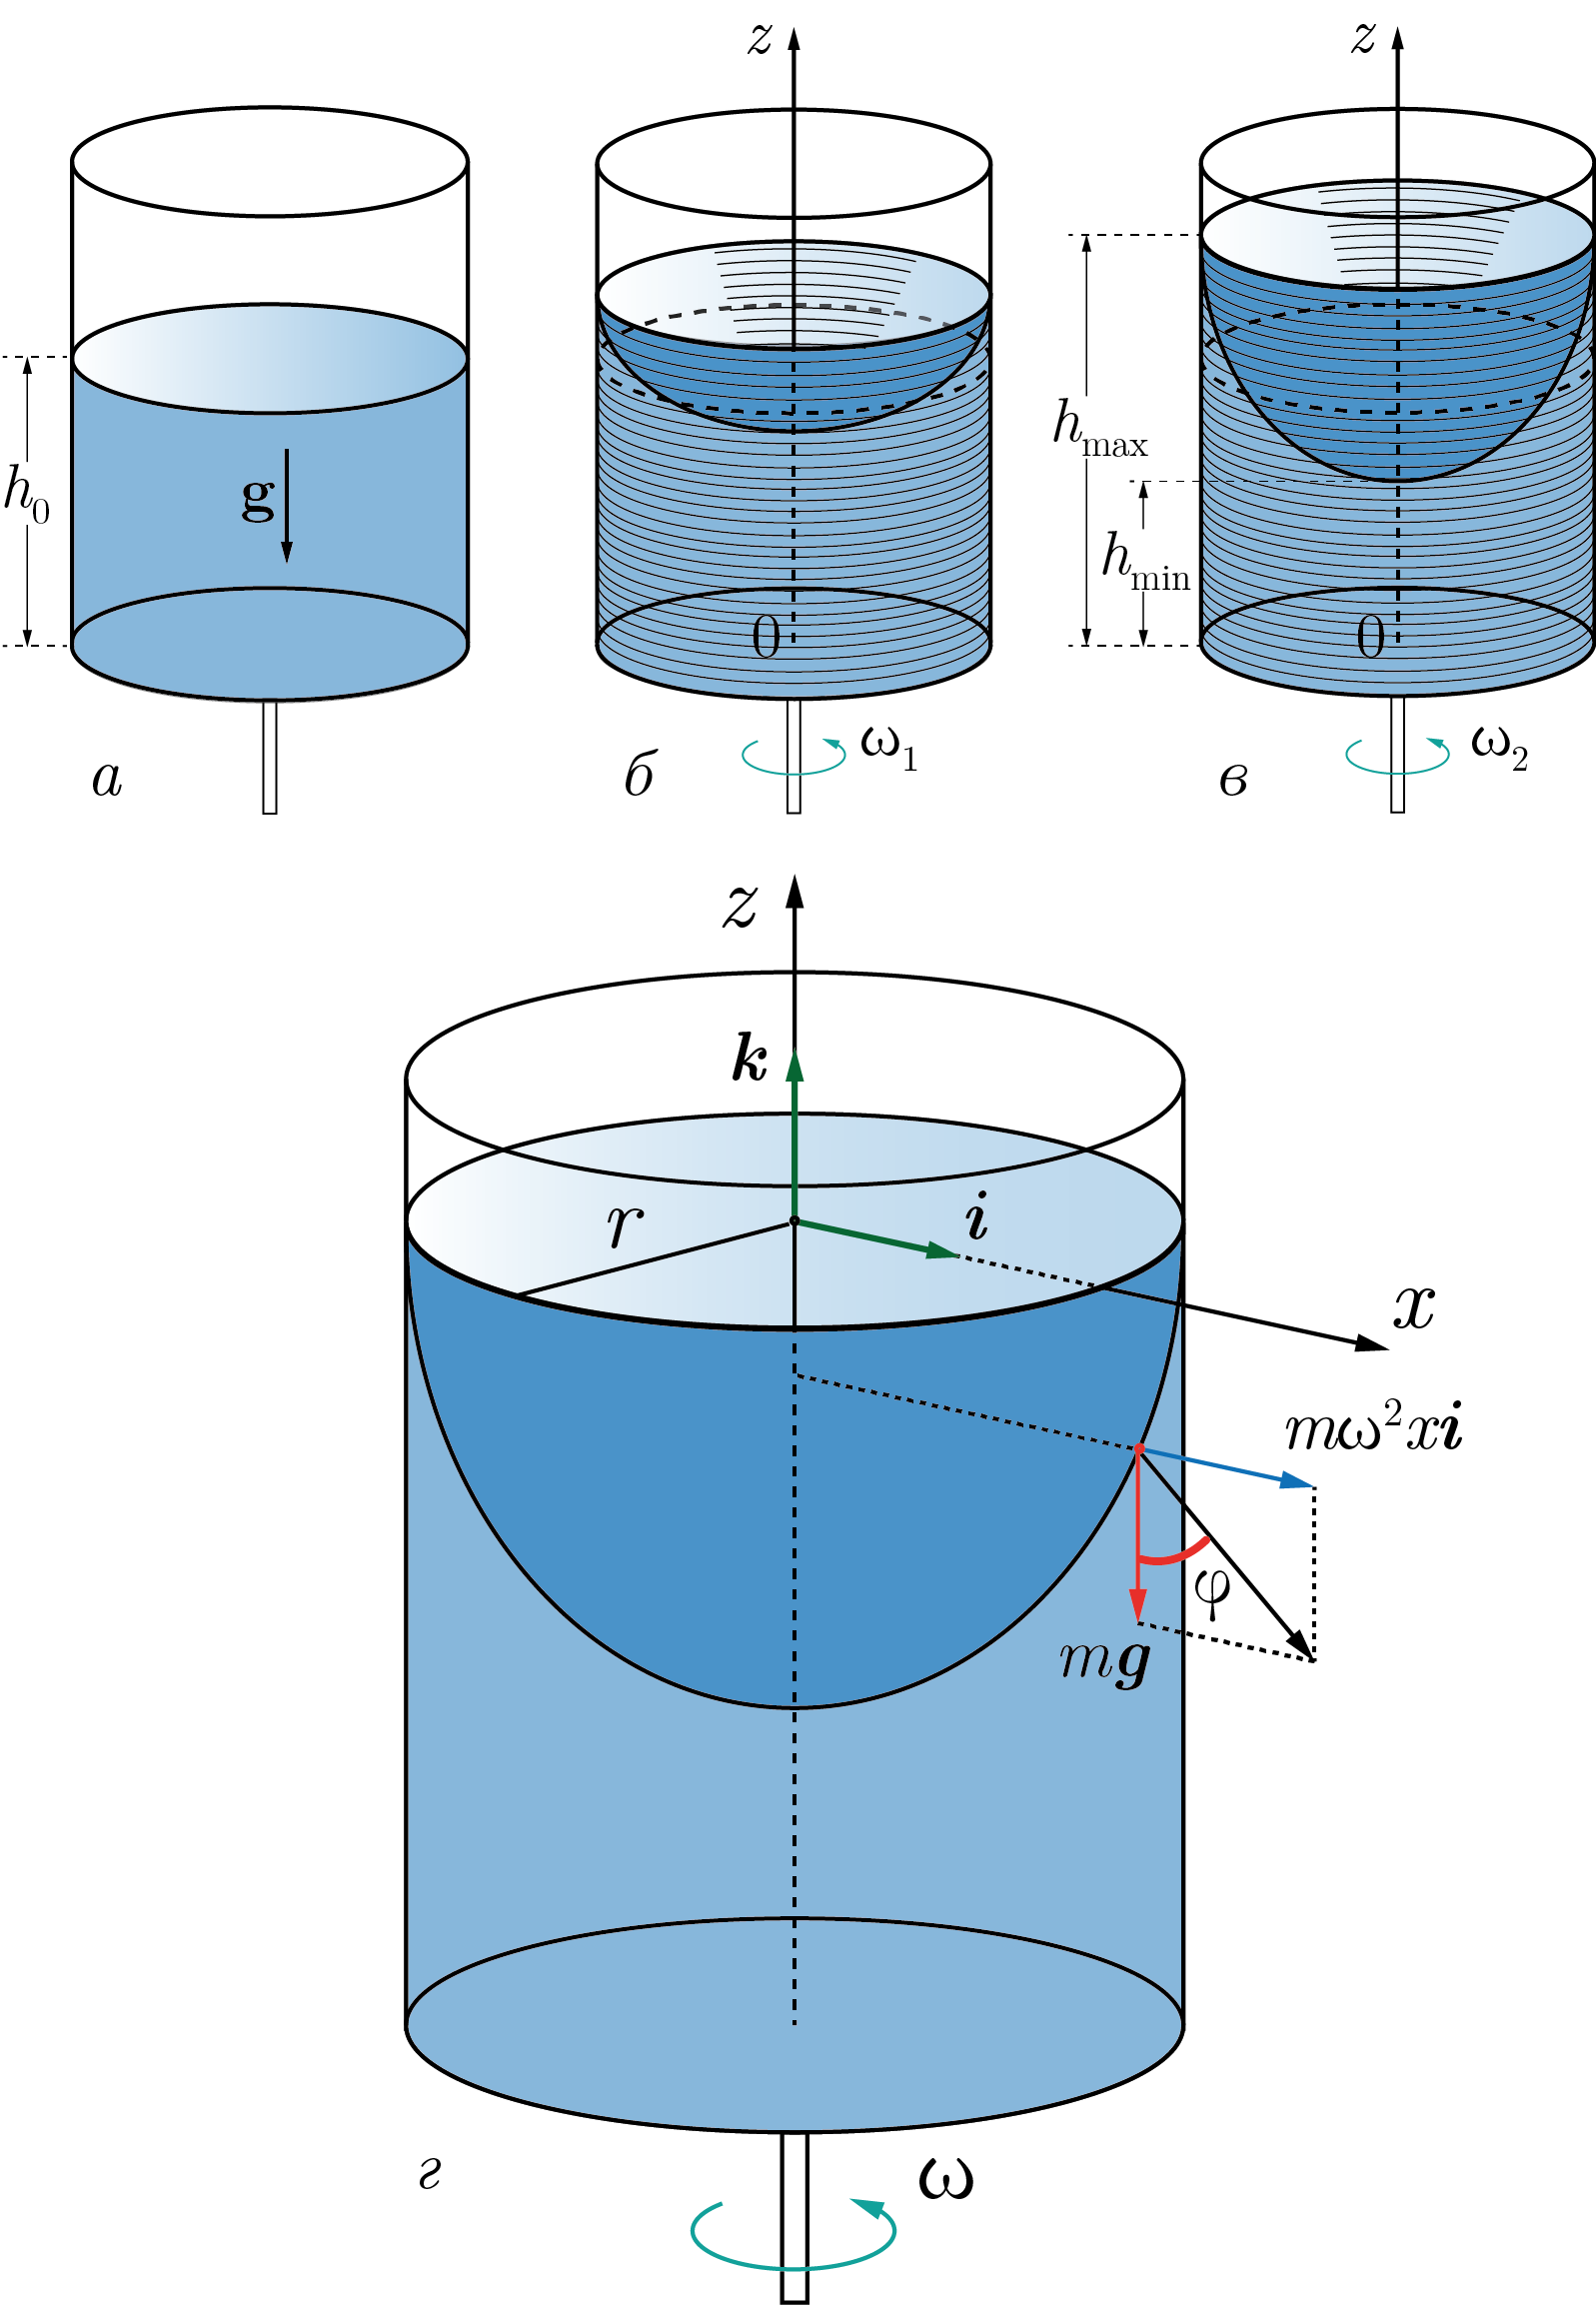
\includegraphics[width=0.6\linewidth]{paraboloid-3.png}
	\caption{Формирование параболоида в жидкости при различной угловой скорости вращения подставки}
	\label{paraboloid-3}
\end{figure}

Таким образом, полную глубину воронки в жидкости
\begin{align}\label{2}
h_{max} - h_{min}= \frac{\omega^{2} r^{2}}{2g}.
\end{align}
можно определить угловую скорость вращения цилиндра.

Подобный эффект, благодаря которому чаинки при перемешивании воды собираются в центре образовавшейся воронки, заключается в следующем.

\begin{figure}[H]
	\centering 	
	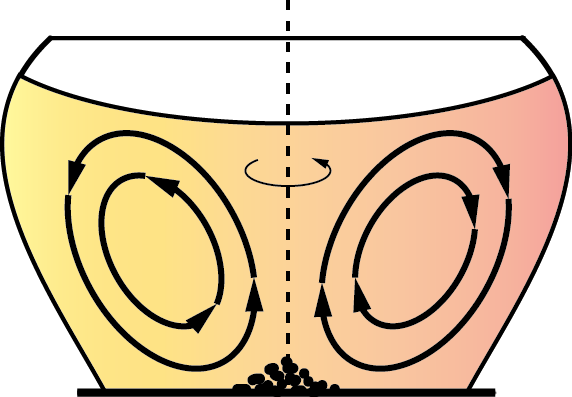
\includegraphics[width=0.45\linewidth]{paraboloid-4.png}
	\caption{Структура течения и поведение чаинок в чашке при вращении жидкости}
	\label{paraboloid-4}
\end{figure}

Когда жидкость начинает вращаться, то благодаря вязкости ее частицы постоянно вовлекается во вращение с возрастающей угловой скоростью. 
Постепенно ускоренные слои жидкости достигают вращающихся чаинок, и тут проявляет себя то обстоятельство, что вода и чаинки имеют разную плотность.
Плотность чаинок больше, а значит, их труднее вовлекать в ускоренное движение, чем расположенные рядом слои жидкости. 
Чаинки отстают от окружающей их жидкости и, следовательно, перемещаются к оси цилиндр.
Если же цилиндр не ускоряется, а тормозится, то все будет происходить наоборот.

\end{document}
